\documentclass[tikz,border=8pt]{standalone}
\usepackage{xcolor}
\usetikzlibrary{arrows.meta,positioning}
\tikzset{
  head/.style={
    draw,
    rounded corners=4pt,
    minimum width=4.7cm,
    minimum height=0.95cm,
    text width=4.5cm,
    align=center,
    font=\small\bfseries,
    fill=gray!10
  },
  process/.style={
    draw,
    rounded corners=4pt,
    minimum width=4.1cm,
    minimum height=0.9cm,
    text width=3.95cm,
    align=center,
    font=\scriptsize,
    fill=blue!8
  },
  store/.style={
    draw,
    rounded corners=4pt,
    minimum width=4.1cm,
    minimum height=0.9cm,
    text width=3.95cm,
    align=center,
    font=\scriptsize,
    fill=green!9
  },
  trace/.style={
    draw,
    rounded corners=4pt,
    minimum width=4.1cm,
    minimum height=0.9cm,
    text width=3.95cm,
    align=center,
    font=\scriptsize,
    fill=purple!10
  },
  flow/.style={->, >=Latex, thick, draw=gray!70}
}
\begin{document}
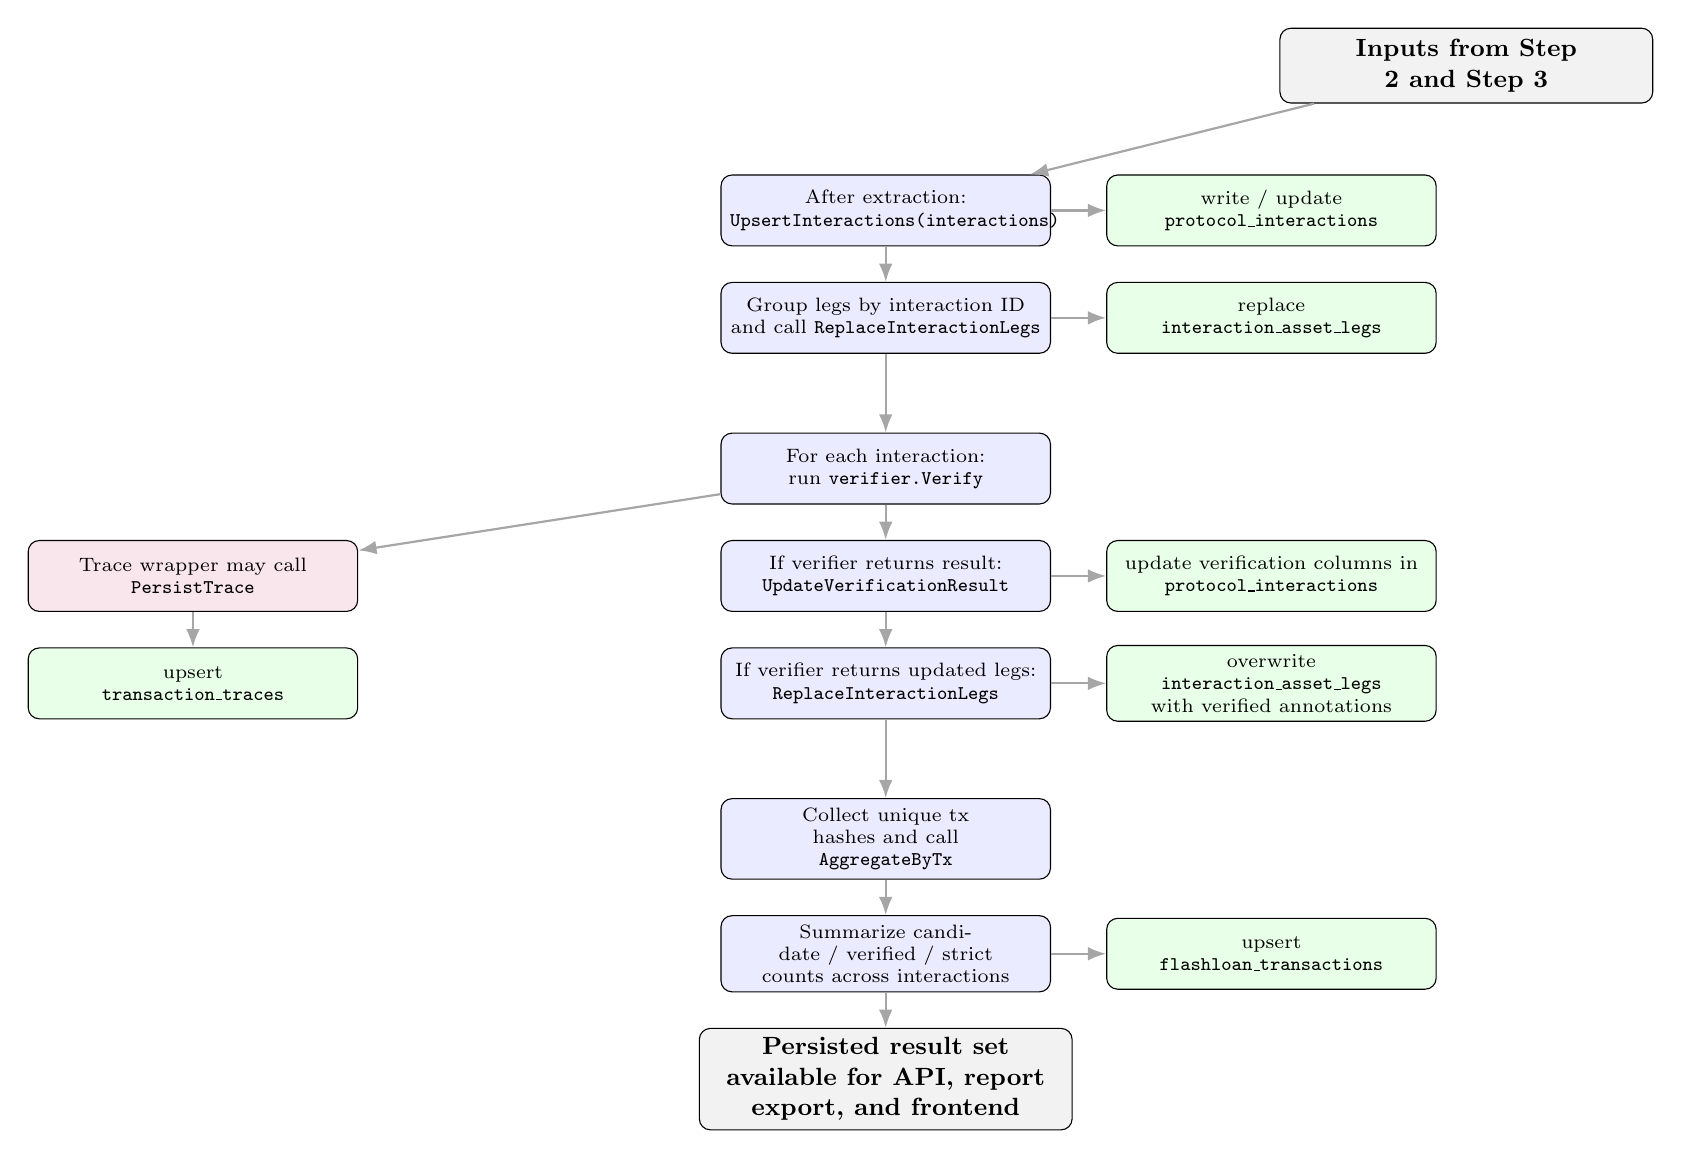
\begin{tikzpicture}[node distance=0.45cm]
  \node[head] (input) at (0,0) {Inputs from Step 2 and Step 3};

  \node[process, below left=0.9cm and 2.9cm of input] (c1) {After extraction:\\\texttt{UpsertInteractions(interactions)}};
  \node[store, right=0.7cm of c1] (s1) {write / update\\\texttt{protocol\_interactions}};
  \node[process, below=of c1] (c2) {Group legs by interaction ID\\and call \texttt{ReplaceInteractionLegs}};
  \node[store, right=0.7cm of c2] (s2) {replace\\\texttt{interaction\_asset\_legs}};

  \node[process, below=1.0cm of c2] (v1) {For each interaction:\\run \texttt{verifier.Verify}};
  \node[process, below=of v1] (v2) {If verifier returns result:\\\texttt{UpdateVerificationResult}};
  \node[store, right=0.7cm of v2] (s3) {update verification columns in\\\texttt{protocol\_interactions}};
  \node[process, below=of v2] (v3) {If verifier returns updated legs:\\\texttt{ReplaceInteractionLegs}};
  \node[store, right=0.7cm of v3] (s4) {overwrite\\\texttt{interaction\_asset\_legs}\\with verified annotations};

  \node[trace, left=4.6cm of v2] (t1) {Trace wrapper may call\\\texttt{PersistTrace}};
  \node[store, below=of t1] (t2) {upsert\\\texttt{transaction\_traces}};

  \node[process, below=1.0cm of v3] (a1) {Collect unique tx hashes and call\\\texttt{AggregateByTx}};
  \node[process, below=of a1] (a2) {Summarize candidate / verified / strict\\counts across interactions};
  \node[store, right=0.7cm of a2] (s5) {upsert\\\texttt{flashloan\_transactions}};

  \node[head, below=of a2] (output) {Persisted result set available for API, report export, and frontend};

  \draw[flow] (input) -- (c1);
  \draw[flow] (c1) -- (s1);
  \draw[flow] (c1) -- (c2);
  \draw[flow] (c2) -- (s2);
  \draw[flow] (c2) -- (v1);
  \draw[flow] (v1) -- (v2);
  \draw[flow] (v2) -- (s3);
  \draw[flow] (v2) -- (v3);
  \draw[flow] (v3) -- (s4);
  \draw[flow] (v1) -- (t1);
  \draw[flow] (t1) -- (t2);
  \draw[flow] (v3) -- (a1);
  \draw[flow] (a1) -- (a2);
  \draw[flow] (a2) -- (s5);
  \draw[flow] (a2) -- (output);
\end{tikzpicture}
\end{document}
